% Created 2021-12-28 Tue 12:21
% Intended LaTeX compiler: pdflatex
\documentclass[11pt]{article}
\usepackage[utf8]{inputenc}
\usepackage[T1]{fontenc}
\usepackage{graphicx}
\usepackage{longtable}
\usepackage{wrapfig}
\usepackage{rotating}
\usepackage[normalem]{ulem}
\usepackage{amsmath}
\usepackage{amssymb}
\usepackage{capt-of}
\usepackage{hyperref}
\author{Ian Gomez}
\date{\today}
\title{Visualizing Data Using t-SNE}
\hypersetup{
 pdfauthor={Ian Gomez},
 pdftitle={Visualizing Data Using t-SNE},
 pdfkeywords={},
 pdfsubject={},
 pdfcreator={Emacs 27.1 (Org mode 9.6)}, 
 pdflang={English}}
\begin{document}

\maketitle
\tableofcontents


\section{Abstract}
\label{sec:org90bb8c3}
TSNE visualizes high dimensional data by giving a location in a 2d/3d mapping.
Improves on previous visualizations by reducing the crowind problem
Through the use of random walks it is possible to use this \(O(n^2)\) algorithm for large datasets
\section{Introduction}
\label{sec:org011a839}
\begin{itemize}
\item Previous visualization techniques only allow the user to display the data in 2d/3d but leave the interpretation to the user.
\item The goal of dimensionality reduction methods is to reduce the high dimensional data of \(X = \{x_1...x_n\}\) to a set of points \(Y = \{y_1...y_n\}\)
\item every \(y_i\) is referred to as a map point. The aim of dimensionality reduction techniques is to preserve the significant structure of the data (e.g. relative distances between points like in random projection).
\item Most techniques tend to not keep both global and local structures using a single mapping.
\end{itemize}
\section{Stochastic Neighbor Embedding (SNE)}
\label{sec:orge00d24f}
\begin{itemize}
\item Converts high dimensional euclidean distances into conditional probablistic distances (similarities)
\item Each similarity represents the probability of point \(x_i\) to chose point \(x_j\) as a neighbor using a gaussian distribution. It is represented as \(p_{j|i}\).
\item the probability is computed using the formula \(p_{j|i} = \frac{exp(-||x_i-x_j||^2/\sigma^2)}{\sum_{k \neq i}(-||x_i - x_k||^2/\sigma^2)}\)
\item Computes the probability of getting \(x_j\) normalized over the probability of all points
\item We can also do this for the low dimensional mapping for all \(y_i\) and all \(y_j\)
\item Where the probability distribution will be notated as \(q_{j|i}\) and the computation is the same for the high dimensional case but using the low dimensional points. And the variance is set to \(1/\sqrt2\)
\item For all points where \(i=j\) we set the probability to 0.
\item The goal of SNE is to minimize the distance (mismatch) between P and Q. Thus we intuitively use the KL-divergence formula for the loss function
\item To solve this we compute the sum of all KL divergences for each conditional P and Q probability
\item \(C = \sum_iKL(P_i||Q_i)\) where \(P_i\) and \(Q_i\) are the marginalized probability for each \(x_i\), \(y_i\)
\item Because of the KL divergence being non-symmetric the loss penalizes far \(y_i\) which are close in \(x_i\) more than close points in \(y_i\) which are far in \(x_i\).
\item Analytically it penalizes high \(P_i\) and low \(Q_i\).
\item This can be viewed as having high attraction gradients and low repulsion gradients
\item In turn the SNE function focuses more on keeping local structures in the data mapping.
\item Now when determining the Gaussian we need a way to select the variance. To do this we define perplexity.
\item \(Perp(P_i) = 2^{H(P_i)}\)
\item where \(H(P_i)\) is the shannon entropy of a probability distribution measured in bits (log\textsubscript{2})
\item Finally to select the variance we perform a binary search until we get to the given perplexity that is specified by the user.
\item This perplexity is essentially a smooth measure of the number of neighbors we assume is in the neighborhood. However, performance is pretty robust to this number, and is usually designated between 5 and 50.
\item As mentioned previously the gradient can be thought of as an attraction or repulsion of points depending on the distance after mapping. (there is more explanation of this interpretation on the paper)
\item For the optimization algorithm we first sample random \(y_i\) from an Isotopic Gaussian that has a small variance.
\item We also add a momentum term so that we can skip over poor local optima.
\item Finally Gaussian noise is added into the map point, and the variance of this noise is decreased later through the process.
\item Thus SNE tends to have a difficult optimization process, and requires multiple runs to get good visualizations after hyperparameter tuning. Since this is a non-convex optimization problem.
\end{itemize}
\section{t-Distributed SNES (t-SNE)}
\label{sec:orgd7d0cb6}
\begin{itemize}
\item the main problems of SNE are the difficulty of optimization, and the ``crowding problem''.
\item Therefore for t-SNE we will solve this using symmetric SNE with a simple gradient and a student t-Distribution for a heavy-tailed distribution to alleviate the crowding problem and the optimization of SNE.
\end{itemize}
\section{Symmetric SNE}
\label{sec:org5aab0a8}
\begin{itemize}
\item An alternative to solving the original KL divergence is that we can instead minimize a KL divergence over the joint probability of P and Q. In this case we get
\item \(KL(P||Q) = \sum_i \sum_j p_{ij}log(\frac{p_{ij}}{q_{ij}})\)
\item In this case each \(p_{ij} = p_{ji}\) and the same for q, also we set \(p_{ii}\) to 0.
\item Therefore for each \(q_{ij}\) we compute
\item \(q_{ij} = \frac{exp(-||y_i-y_j||^2)}{\sum{k \neq l}(-||y_k - y=l||^2)}\)
\item (Note that the difference here is that the summation is over all pairwise points as opposed to all points conditional to \(y_i\))
\item Intuitively we would do this for all \(x_i\) however, this causes the problem that when the \(x_i\) is an outlier it will have almost no effect on the location of the \(y_i\) since it is almost irrelavent to the normalization constant
\item Therefore we use \(P_{ij} = \frac{p_{j|i}+p_{i|j}}{2n}\)
\item This allows the margenalization of \(\sum_j p_{ij} > \frac{1}{2n}\). Thus making each datapoint have a significant contribution to the gradient.
\item Another benefit of symmetric SNE is that the form of the gradient is simpler.
\item \(\frac{\delta C}{\delta y_i}=4\sum_j(p_{ij}-q_{ij})(y_i-y_j)\)
\item Symmetric SNE seems to perform as well if not better than regular SNE
\end{itemize}
\section{The Crowding problem}
\label{sec:orga910985}
\begin{itemize}
\item The main point of the crowding problem is that in the high dimensional space there are more points exist that are equidistant. Because of this that means each point will in turn have more neighbors as the dimensionality increases. Which leads to points clumping together in the lower level representation
\item If we were to reduce the dimensionality the data we would need to increase the distance to make the distances very far, however, since there are so many equidistant points in the high dimensional space they will eventually converge through the sheer amount of equidistant points.
\item One idea is to add a repulsion factor to the gradient with a uniform distribution with a mixing proportion. So that the values of \(q_{ij}\) cannot fall below \(\frac{2\rho}{\rho (n-1)}\)
\item This ensures that the values of \(q_{ij}\) that are far apart in the high dimensional space will have values of \(q_{ij}\) that are always larger than \(p_{ij}\).
\item However, this uniform sne called (UNI-SNE) is tedious. Also due to this repulsive effect if two parts of a cluster get seperated early there is not a strong enough attractive force to pull them together.
\end{itemize}
\section{Mismatched Tails can compensace for Mismatched Dimensionalities.}
\label{sec:org1f1e4b9}
\begin{itemize}
\item The purpose of this section is to explain how using a Gaussian in the high dimensionality case and a t-Distribution in the low dimensionality space can improve performance.
\item The t-Distribution allows use to model moderate distances in the high-dimensional space to be modeled by a larger distance in the low-dimensional space.
\item The reason we use the t-Distribution is because it has a heavier density in the tails than a standard gaussian.
\item We specifically use 1 degree of freedom for our t-Distribution
\item therefore we define each \(q_{ij}\) as
\item \(q_{ij} = \frac{(1+||y_i-y_j||^2)^{-1}}{\sum_{k \neq l}(1+||y_k - y_l||^2)^{-1}}\)
\item By using a single degree of freedom our similarities have an inverse square law in respect to the pairwise distances.
\item Another important note is that the t-distribution is invariant to changes of scale for map points that are far apart (reducing the size of gradients). Finally it makes it so that large clusters of points that are far apart interact just like individual points.
\item The reason for choosing the t-distribution is that it is similar to a gaussian since it is just an infinite mixture of Gaussians. Also it is much faster to evaluate computationally due to the lack of an exponential function.
\item The gradient is \(\frac{\delta C}{\delta y_i} = 4 \sum_j (p_{ij}-q_{ij}) (y_i-y_j) (1+||y_i-y_j||^2)^{-1}\)
\item Some of the benefits of this optimization is that t-SNE strongly repels dissimilar datapoints that have a small distance in Y and large distance in X.
\item SNE and UNI-SNE have this as well. For SNE the relative size in compared to the attraction gradient size is irrelavent. For UNI-SNE the values are only large if the points are already far apart (which is rarely the case due to the gaussian sampling).
\item Also since t-SNE has a strong repulsion it does not go to infinity which is different from UNI-SNE, since very disimilar datapoints in the high dimensional maps will have extremely large repulsion gradients.
\item t-SNE also adds long range forces due to the large tail density, which also allows for points which are seperated early to get pulled back together since the distance does not introduce a exponential decay of force.
\item This allows the ability to find good local optima without the addition of gaussian noise
\end{itemize}
\section{Optimization methods for t-SNE}
\label{sec:org85c5112}
\begin{itemize}
\item For t-SNE we use momentum and adaptive learning rates to improve the quality of the local minima.
\item We can also use ``early compression'' so that points stay close together during the early stages of optimization.
\item Early compression is essentially adding an L2 regularization term which gets removed after a user set amount of iterations.
\item Another trick that is used is called ``early exaggeration'' to multiply the \(p_{ij}\) by a constant value in early stages of optimization.
\item Therefore since the \(q_{ij}\) still add up to 1 the \(q_{ij}\) is not large enough to model the \(p_{ij}\). This means that the algorithm will first try to create large cluster distances due to the really large \(p_{ij}\).
\item This is the algorithm provided by the paper.
\end{itemize}
\begin{center}
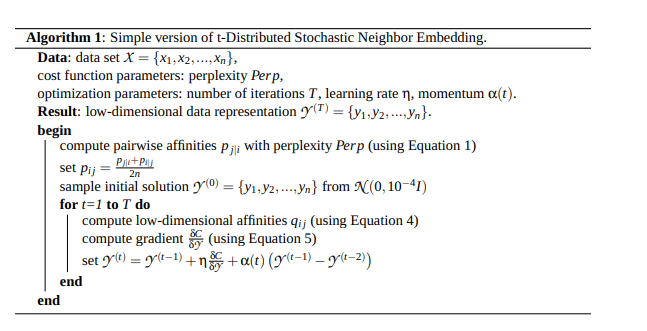
\includegraphics[width=.9\linewidth]{./images/tsne_algo.png}
\end{center}

\section{For the next sections I will just give a brief overview of the sections since it discusses results and extra discussion that I don't currently want to write about.}
\label{sec:org93594f5}

\section{Experiments}
\label{sec:org679687d}
\begin{itemize}
\item Compares t-SNE to different SOTA visualization algorithms (Further discussed in paper)
\end{itemize}
\section{Applying t-SNE to Large Data sets}
\label{sec:org9a140ff}
\begin{itemize}
\item Applies a random walk algorithm to find landmarks and extra points to compute \(p_{j|i}\)
\item This can be run either through performing the random walks or through an analytical solution. However in practice these both work about the same.
\item It may be better to use the analytical solution for very large datasets.
\end{itemize}
\section{Comparison with different techniques.}
\label{sec:org7a098f9}
\begin{itemize}
\item Talks about how the algorithm compares to different visualization techniques and how it solves/outperforms some of the problems that other techniques have.
\end{itemize}
\section{Weaknesses}
\label{sec:org84cbaf4}
\begin{itemize}
\item t-SNE has 3 potential weaknesses
\item 1. unproven general dimensionality reduction for dimensions > 3d
\item 2. Relative local nature of t-SNE makes it sensitve to dimensionality of the data.
\item 3. not guaranteed to converge to global optimum
\end{itemize}
\end{document}
